\section*{VPN (Virtual Private Networks)}

\large As VPNs \textbf{Virtual Private Networks} são túneis pela qual o tráfego da internet passa para que o IP original do usuário não seja exposto, dificultando o trabalho de governos e por pessoas mal intencionadas.\\

	VPNs não são usadas pela maioria dos usuários, alguns por dificuldade em usa-las e outros por simplesmente não conhecer o que são VPNs. Mas ao contrário que muitos usuários pensam, é simples e rápido configurar uma VPN.

\begin{center}
	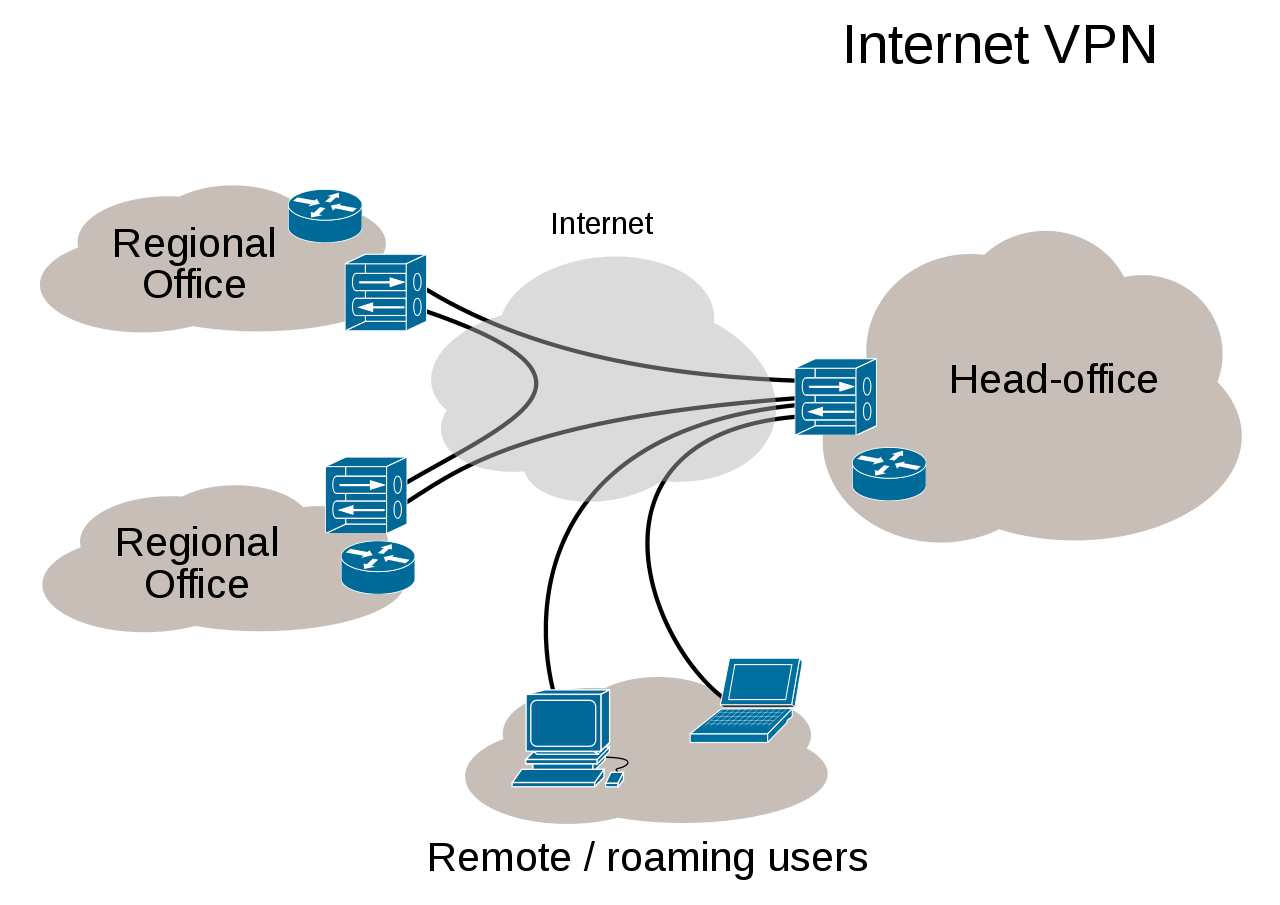
\includegraphics[scale=1]{vpn.png}
\end{center}


O \href{https://openvpn.org/}{OpenVPN} é o cliente VPN mais conhecido e usado atualmente. Ele é um software livre que serve para criar VPN e também para se conectar à servidores VPNs e é o mais recomendado de se usar pela sua facilidade de uso como também pela segurança. OpenVPN é multriplataforma e está disponível para distribuições Linux, MacOS e Windows.
